\documentclass{article}
\usepackage[utf8]{inputenc} %кодировка
\usepackage[T2A]{fontenc}
\usepackage[english,russian]{babel} %русификатор 
\usepackage{mathtools} %библиотека матеши
\usepackage[left=1cm,right=1cm,top=2cm,bottom=2cm,bindingoffset=0cm]{geometry} %изменение отступов на листе
\usepackage{amsmath}
\usepackage{graphicx} %библиотека для графики и картинок
\graphicspath{}
\DeclareGraphicsExtensions{.pdf,.png,.jpg}
\usepackage{subcaption}
\usepackage{pgfplots}
\usepackage{float}
\usepackage{hyperref}


\begin{document}
% НАЧАЛО ТИТУЛЬНОГО ЛИСТА
\begin{center}
    \Large
    Федеральное государственное автономное \\
    образовательное учреждение высшего образования \\ 
    «Научно-образовательная корпорация ИТМО»\\
    \vspace{0.5cm}
    \large
    Факультет программной инженерии и компьютерной техники \\
    Направление подготовки 09.03.04 Программная инженерия \\
    \vspace{1cm}
    \Large
    \textbf{Отчёт по лабораторной работе №2} \\
        По дисциплине «Бизнес логика программных систем» ( семестр 6)\\
    \large
    \vspace{8cm}

    \begin{minipage}{.33\textwidth}
    \end{minipage}
    \hfill
    \begin{minipage}{.4\textwidth}
    
        \textbf{Студент}: \vspace{.1cm} \\
        \ Дениченко Александр\\
        \ Разинкин Александр\\
        \textbf{Преподаватель}:  \\
        \ Бобрусь Александр
    \end{minipage}
    \vfill
Санкт-Петербург\\ 2025 г.
\end{center}
\pagestyle{empty}
% КОНЕЦ ТИТУЛЬНОГО ЛИСТА 
\newpage
\pagestyle{plain}

\section*{Данные}
Доработать приложение из лабораторной работы \#1, реализовав в нём управление транзакциями и разграничение доступа к операциям бизнес-логики в соответствии с заданной политикой доступа.
\\
Управление транзакциями необходимо реализовать следующим образом:

Переработать согласованные с преподавателем прецеденты (или по согласованию с ним разработать новые), объединив взаимозависимые операции в рамках транзакций.

Управление транзакциями необходимо реализовать с помощью Spring JTA.

В реализованных (или модифицированных) прецедентах необходимо использовать декларативное управление транзакциями.

В качестве менеджера транзакций необходимо использовать Jakarta EE JTA, предварительно преобразовав приложение в war, развёртываемый на сервере приложений WildFly.

Разграничение доступа к операциям необходимо реализовать следующим образом:
\\
Разработать, специфицировать и согласовать с преподавателем набор привилегий, в соответствии с которыми будет разграничиваться доступ к операциям.

Специфицировать и согласовать с преподавателем набор ролей, осуществляющих доступ к операциям бизнес-логики приложения.

Реализовать разработанную модель разграничений доступа к операциям бизнес-логики на базе Spring Security. Информацию об учётных записах пользователей необходимо сохранять в реляционую базу данных, для аутентификации использовать JWT.

\section*{Модель потока управления}
\url{https://drive.google.com/file/d/1cPEd-fhmsBNOvO_BABxoh9T3XESQbnIZ/view?usp=sharing}

\section*{Спецификация пользовательских привилегий и ролей}
USER - обычный человек, который может делать заказы\\
CUSTOMER - продавец, есть доп функционал по размещению товаров и принятия решений по поводу заказов
\\ADMIN - может просматривать профили людей, смотреть списки на получение админских прав, и ставить баланс пользователям

\section*{Спецификация REST API}
\begin{center}
    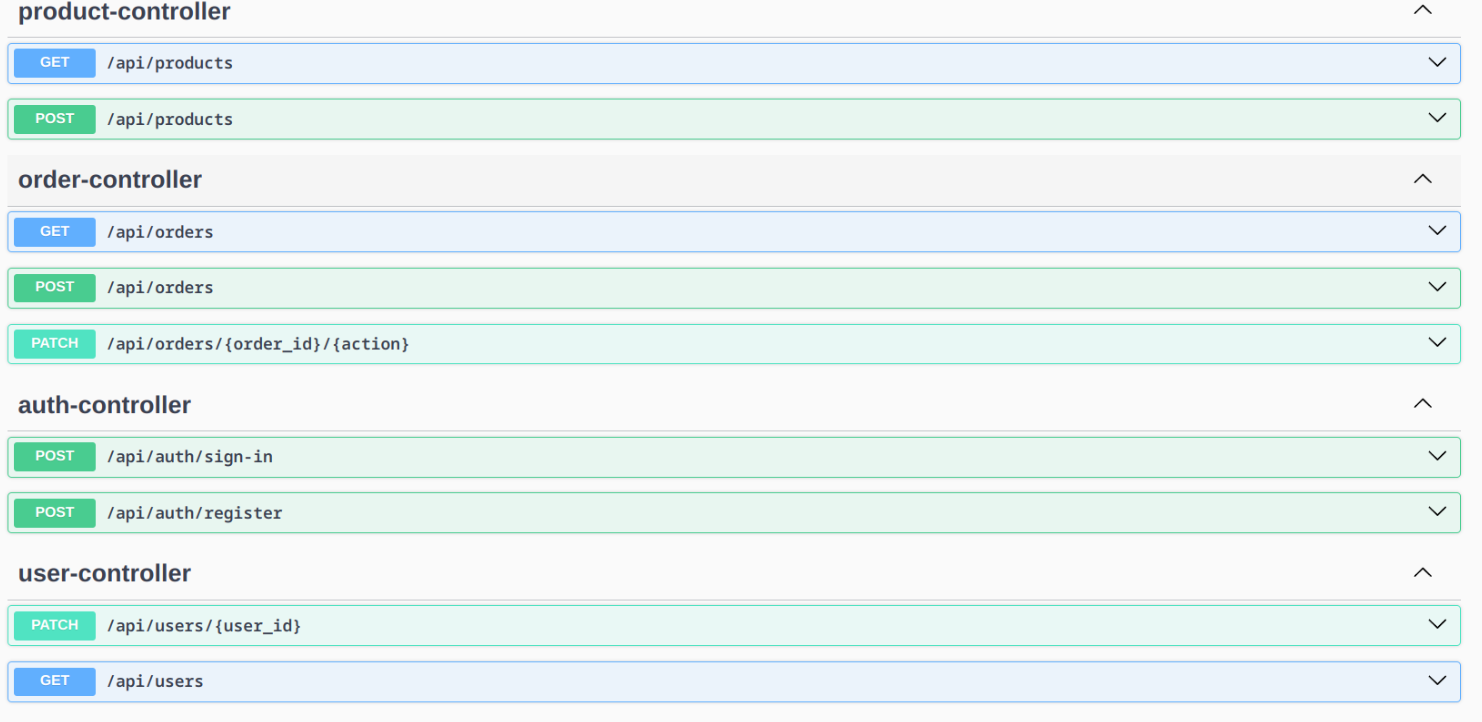
\includegraphics[width=.9\textwidth]{1}
\end{center}
\begin{center}
    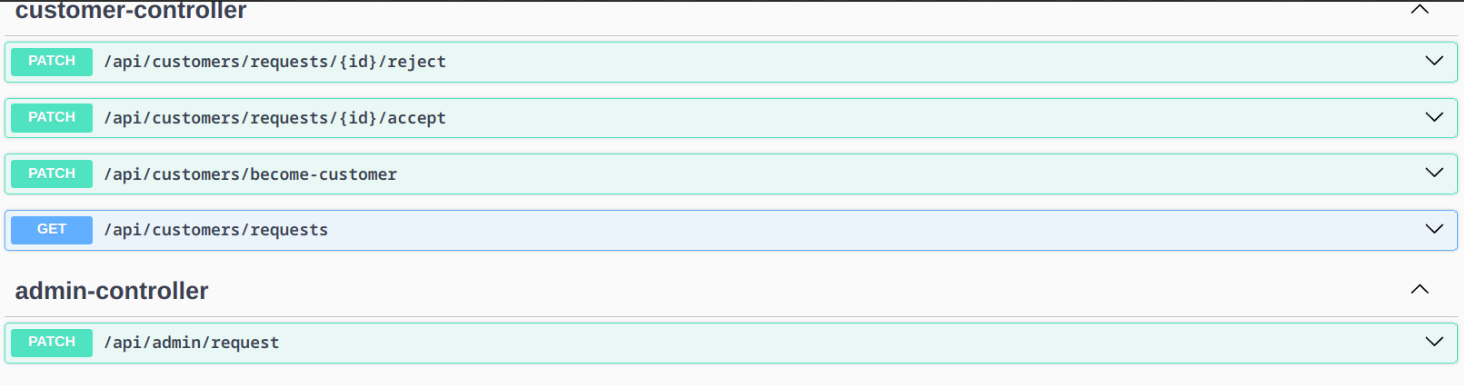
\includegraphics[width=.9\textwidth]{2}
\end{center}
\section*{Исходный код системы}
\url{https://github.com/DecafMangoITMO/blps_lab1}

\section*{Вывод}
В результате доработки приложения из лабораторной работы №1 удалось реализовать два ключевых аспекта: управление транзакциями и разграничение доступа к операциям бизнес-логики.
Было успешно интегрировано с помощью Spring JTA и Jakarta EE JTA, что обеспечило надёжность и целостность данных при выполнении взаимозависимых операций.
Реализовано на базе Spring Security с использованием JWT для аутентификации и реляционной базы данных для хранения учётных записей пользователей, что повысило безопасность и гибкость системы.

\end{document}
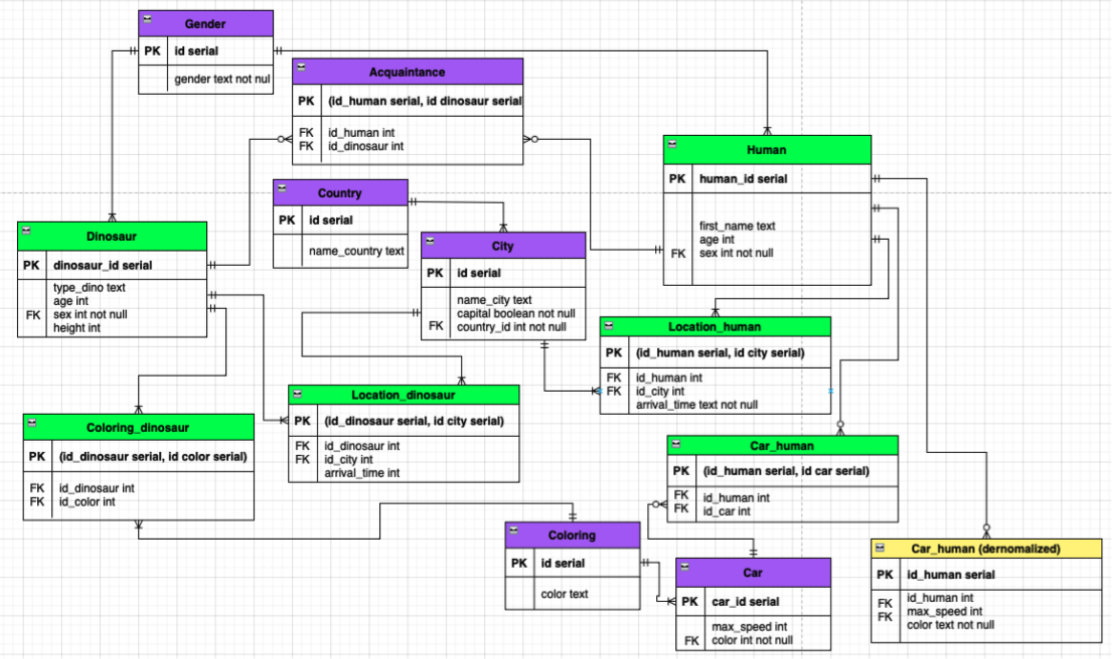
\includegraphics[width=.9\textwidth]{123}